\newpage
\question~\\
\begin{center}
        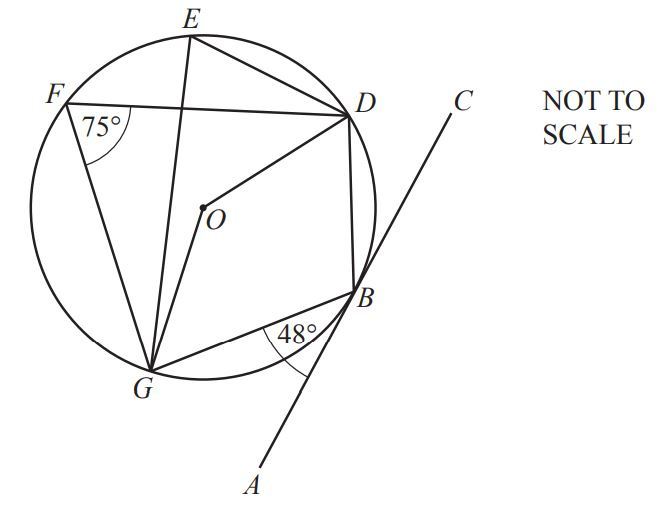
\includegraphics[scale=0.6]{Questions/quiz 19/images/9.JPG}
\end{center} 
In triangle $A C D, B$ is the midpoint of $A C$ and $E$ is the midpoint of $A D$.\\ $\overrightarrow{A B}=6 \mathbf{a}+3 \mathbf{b}$ and $\overrightarrow{D C}=5 \mathbf{a}+2 \mathbf{b}$\\
\begin{parts}
\part Express, as simply as possible, in terms of $\mathbf{a}$ and $\mathbf{b}$.
\begin{itemize}
    \item[(i)] $\overrightarrow{A C}$ \\ \\
    {\flushright{
\hfill          $\overrightarrow{A C}=$ \makebox[12em]{\dotfill}  [1]}}\\ \\

\item[(ii)] $\overrightarrow{A D}$ \\ \\
    {\flushright{
\hfill         $\overrightarrow{A D}=$ \makebox[12em]{\dotfill}  [1]}}
\end{itemize}
\part Show that $\overrightarrow{E B}$ is parallel to $\overrightarrow{D C}$.\\ \\
\makebox[38em]{\dotfill}\\  \\
\makebox[38em]{\dotfill}\\ \\
\makebox[38em]{\dotfill}\\ \\
{{\makebox[38em]{\dotfill}  [3]}}
\end{parts}